%============================================================
%  Capitolo 5 – Ottimizzazione
%============================================================
\chapter{Ottimizzazione}
\label{ch:optimization}

L'ottimizzazione è il processo che permette alla rete neurale di apprendere,
aggiornando iterativamente i parametri $\mathbf{w}$ in modo da minimizzare la
funzione di perdita $\mathcal{L}$. A differenza dell'ottimizzazione classica, in
Deep Learning la funzione obiettivo è \emph{non convessa}, ad alta dimensionalità
e valutatata su dati rumorosi campionati in mini-batch. La comprensione della
geometria della superficie di errore e dei metodi per percorrerla efficientemente
è fondamentale tanto quanto la scelta dell'architettura \citep{bishop2024}.

%------------------------------------------------------------
\section{La Superficie di Errore}
\label{sec:error-surface}

\subsection{Neuroni Lineari e Ciotola Quadratica}
\label{subsec:quadratic-bowl}

La \textbf{superficie di errore} vive in uno spazio con un asse orizzontale per
ogni peso e un asse verticale per il valore della loss. Per un neurone lineare
con errore quadratico medio la superficie è una \textbf{ciotola quadratica}
(quadratic bowl):

\begin{itemize}
  \item Le sezioni verticali sono \textbf{parabole}.
  \item Le sezioni orizzontali sono \textbf{ellissi} (o cerchi se il problema
        è ben condizionato).
\end{itemize}

Per reti multi-layer non lineari la superficie è molto più complessa, ma
\emph{localmente} una ciotola quadratica rimane un'ottima approssimazione.

\begin{figure}[H]
  \centering
  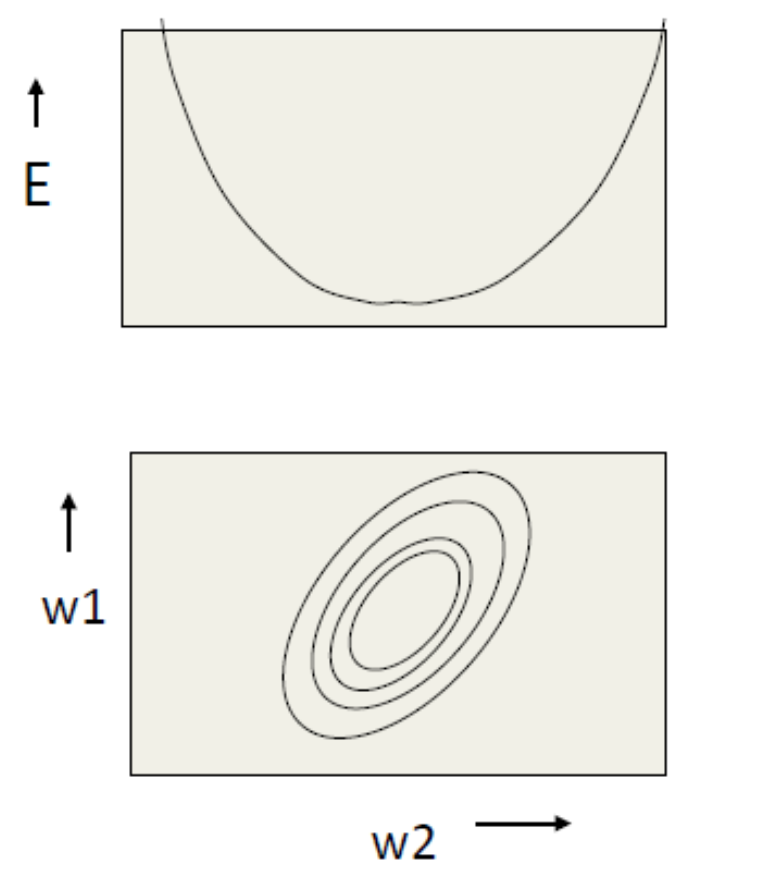
\includegraphics[width=0.72\linewidth]{figures/cf05_error_surface_bowl.png}
  \caption{Sinistra: sezione verticale della superficie di errore per un
           neurone lineare (parabola). Destra: sezione orizzontale (ellissi
           concentriche) nello spazio dei pesi $w_1$--$w_2$.}
  \label{fig:error_surface}
\end{figure}

\subsection{Il Problema della Direzione del Gradiente}
\label{subsec:gradient-direction}

Nella discesa del gradiente si scende lungo la direzione di massima pendenza,
ma questo non coincide con la direzione verso il minimo salvo che le ellissi
siano cerchi. Il problema nasce perché:

\begin{itemize}
  \item Il gradiente è \textbf{grande} nella direzione in cui vogliamo percorrere
        una piccola distanza (curvatura elevata).
  \item Il gradiente è \textbf{piccolo} nella direzione in cui vogliamo percorrere
        una grande distanza (curvatura bassa).
\end{itemize}

Questa asimmetria rende la convergenza lenta e produce i caratteristici
\emph{zig-zag} osservabili nelle traiettorie di ottimizzazione su superfici
ellittiche.

%------------------------------------------------------------
\section{Algoritmi di Apprendimento: Batch, Mini-Batch, Online}
\label{sec:learning-algorithms}

\subsection{Ridondanza nel Dataset}
\label{subsec:redundancy}

Quando il dataset è \textbf{altamente ridondante}, il gradiente calcolato sulla
prima metà dei dati è quasi identico a quello calcolato sulla seconda metà. In
questo caso conviene aggiornare i pesi più volte per epoch, anziché attendere il
calcolo del gradiente completo.

\begin{description}
  \item[Full Batch] Il gradiente viene calcolato sull'intero dataset. Sono
        disponibili metodi più sofisticati (gradiente coniugato non lineare,
        L-BFGS) ma il costo per iterazione è elevato.
  \item[Online (SGD puro)] Il peso viene aggiornato dopo ogni singolo esempio.
        Noisy ma veloce nelle prime fasi.
  \item[Mini-Batch] Compromesso ottimale per reti grandi: si calcola il gradiente
        su un sottoinsieme $B$ di esempi. Sfrutta la moltiplicazione
        matrice-matrice accelerata da GPU e bilancia rumore e costo computazionale.
\end{description}

\paragraph{Regola pratica.}
Per reti neurali grandi su dataset grandi e ridondanti il \textbf{mini-batch} è
quasi sempre la scelta migliore \citep{bishop2024}. I mini-batch devono essere
bilanciati tra le classi per evitare gradienti sistematicamente distorti.

%------------------------------------------------------------
\section{Accorgimenti per il Mini-Batch Gradient Descent}
\label{sec:tricks-minibatch}

\subsection{Learning Rate e Quando Ridurlo}
\label{subsec:lr-schedule}

Abbassare il learning rate $\eta$ durante l'addestramento riduce le fluttuazioni
casuali della loss dovute ai diversi gradienti sui diversi mini-batch:

\begin{itemize}
  \item Si ottiene un \emph{guadagno rapido} nel breve periodo (la loss scende
        più liscia).
  \item Si rallenta però l'apprendimento nel lungo periodo.
\end{itemize}

\begin{figure}[H]
  \centering
  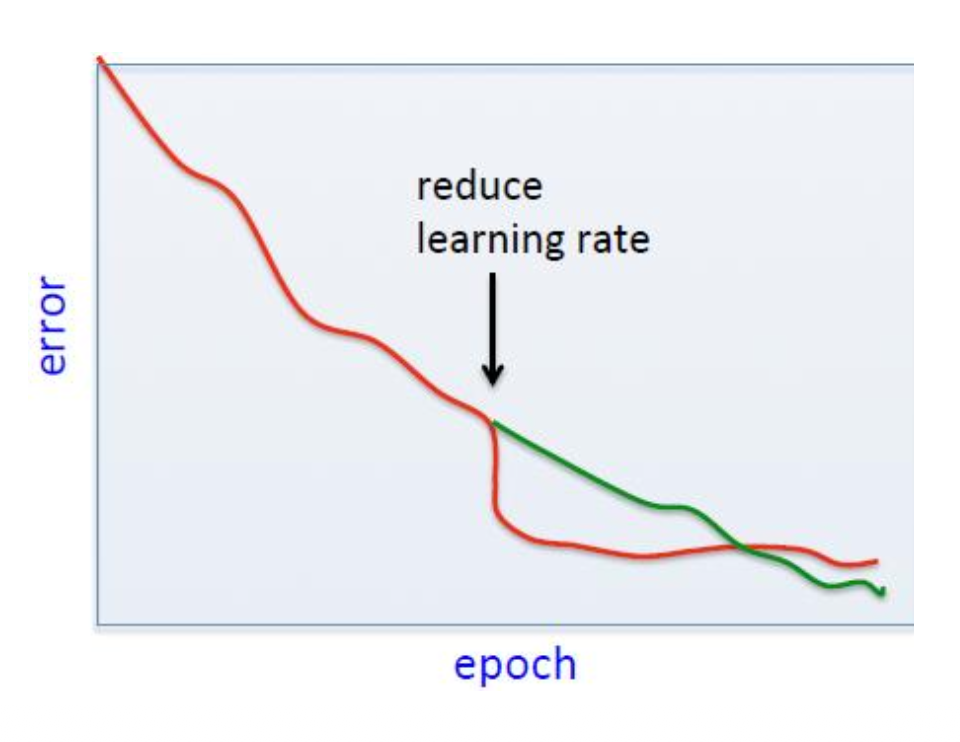
\includegraphics[width=0.60\linewidth]{figures/cf05_lr_schedule.png}
  \caption{Effetto della riduzione del learning rate sulla curva di addestramento.
           La riduzione prematura (rosso) porta a convergenza lenta; quella
           ritardata (verde) sfrutta le oscillazioni iniziali per esplorare meglio
           lo spazio dei parametri.}
  \label{fig:lr_schedule}
\end{figure}

\textbf{Non ridurre il learning rate troppo presto!}

\subsection{Inizializzazione dei Pesi}
\label{subsec:weight-init}

Se due unità nascoste hanno esattamente lo stesso bias e gli stessi pesi in
ingresso e in uscita, riceveranno sempre lo stesso gradiente e non potranno mai
imparare feature diverse. Questo problema, detto \emph{symmetry breaking},
si risolve inizializzando i pesi con valori casuali piccoli.

\paragraph{Fan-in e overshooting.}
Un'unità con fan-in elevato (molti ingressi) può subire un effetto di
\emph{overshoot}: piccole variazioni su molti pesi in ingresso si sommano,
spostando eccessivamente l'uscita. La regola empirica è:

\begin{equation}
  w \propto \frac{\mathcal{N}(0,1)}{\sqrt{n_{\text{in}}}},
\end{equation}

dove $n_{\text{in}}$ è il numero di connessioni in ingresso (fan-in).

\subsubsection{Inizializzazione di Xavier / Glorot}
\label{subsubsec:xavier}

\citet{glorot2010} hanno mostrato che, per preservare la varianza dei segnali
sia in forward che in backward pass, conviene tenere conto sia del fan-in che del
fan-out. Per una distribuzione \textbf{uniforme} $\mathcal{U}(-a, a)$:

\begin{equation}
  a = \text{gain} \times \sqrt{\frac{6}{n_{\text{in}} + n_{\text{out}}}},
\end{equation}

mentre per una distribuzione \textbf{normale} $\mathcal{N}(0, \sigma^2)$:

\begin{equation}
  \sigma = \text{gain} \times \sqrt{\frac{2}{n_{\text{in}} + n_{\text{out}}}}.
\end{equation}

Il parametro \texttt{gain} dipende dalla funzione di attivazione (es.\ $1$ per
la sigmoide, $\sqrt{5}$ per ReLU nella variante He). In PyTorch:
\texttt{nn.init.xavier\_uniform\_} e \texttt{nn.init.xavier\_normal\_}.

\subsection{Pre-elaborazione degli Input}
\label{subsec:input-preprocessing}

Traslare e scalare gli input (\emph{shift and scale}) in modo che abbiano
media zero e varianza unitaria rende la superficie di errore più \emph{circolare}
(meno ellittica), migliorando la velocità di convergenza. Un approccio più
avanzato è la \textbf{decorrelazione} tramite PCA:

\begin{enumerate}
  \item Eliminare le componenti principali con autovalori più piccoli
        (riduzione della dimensionalità).
  \item Dividere le componenti rimanenti per la radice quadrata dei rispettivi
        autovalori (\emph{whitening}).
\end{enumerate}

Per un neurone lineare, il whitening converte la superficie di errore da
un'ellissi allineata agli assi a un cerchio, rendendo ottimale la discesa del
gradiente puro.

%------------------------------------------------------------
\section{Il Metodo del Momentum}
\label{sec:momentum}

\subsection{Intuizione Fisica}
\label{subsec:momentum-intuition}

L'idea del momentum si ispira alla fisica classica: immaginiamo una pallina che
rotola sulla superficie di errore. La posizione della pallina nel piano
orizzontale rappresenta il vettore dei pesi. Inizialmente la pallina segue il
gradiente, ma non appena acquisisce velocità smette di seguire la direzione di
massima pendenza: il \emph{momentum} la trascina nella direzione in cui si stava
già muovendo.

\begin{figure}[H]
  \centering
  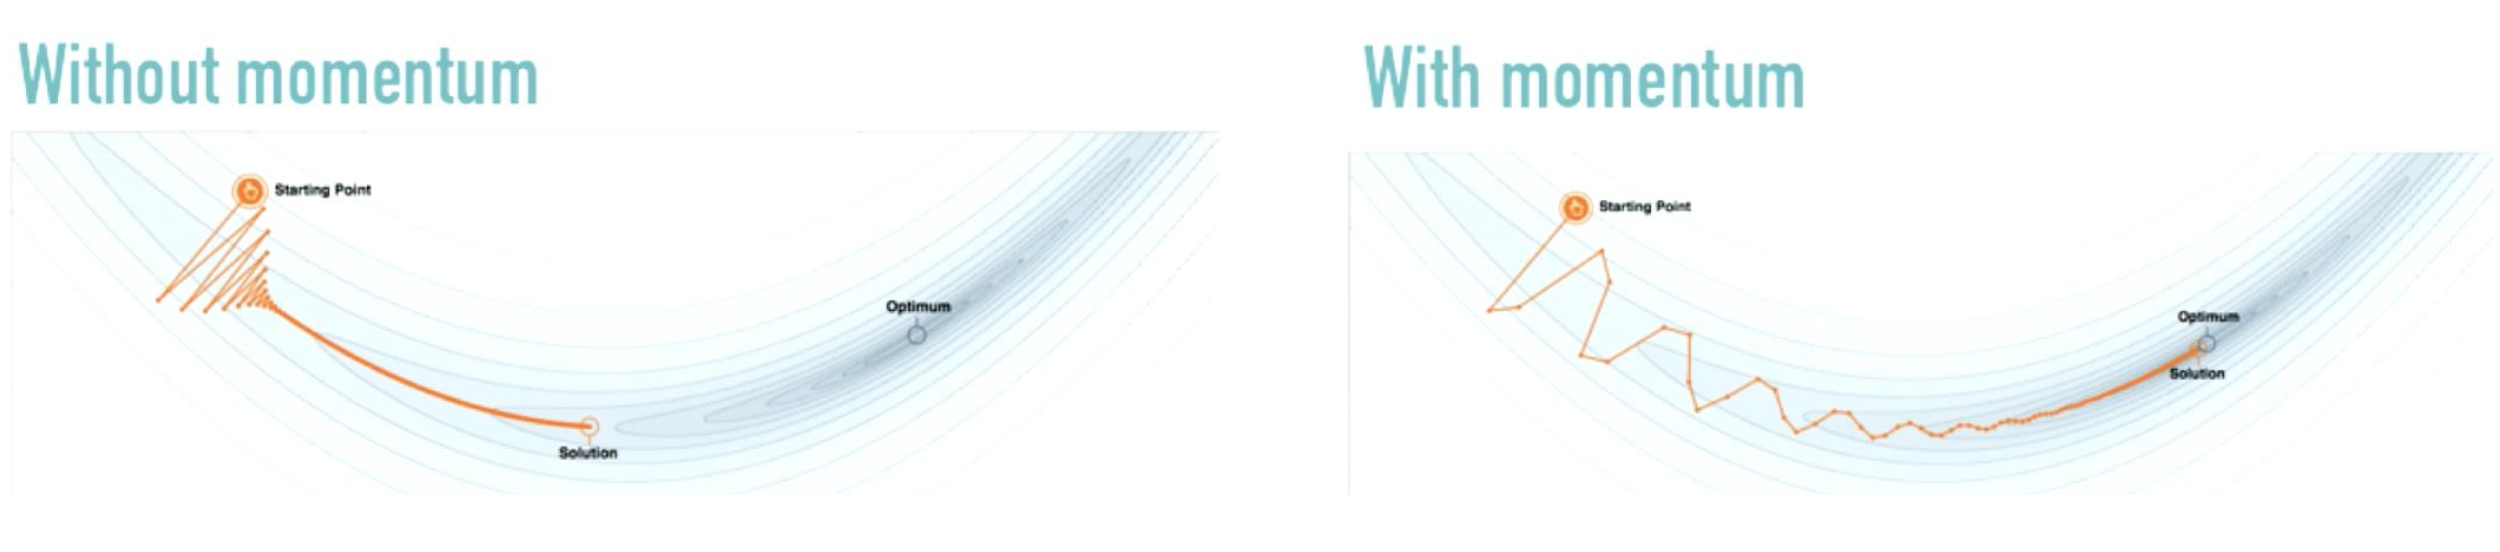
\includegraphics[width=0.75\linewidth]{figures/cf05_momentum_comparison.png}
  \caption{Confronto tra SGD senza momentum (sinistra) e con momentum (destra).
           Senza momentum la traiettoria oscilla fortemente in direzione
           trasversale; con momentum le oscillazioni vengono smorzate e la
           discesa verso il minimo è più diretta.}
  \label{fig:momentum_comparison}
\end{figure}

I benefici principali sono due:
\begin{itemize}
  \item \textbf{Smorzamento delle oscillazioni} nelle direzioni ad alta curvatura,
        combinando gradienti con segno opposto.
  \item \textbf{Accelerazione} nelle direzioni a gradiente piccolo ma consistente.
\end{itemize}

\subsection{Equazioni del Momentum (SGD con Momentum)}
\label{subsec:momentum-equations}

In SGD con momentum si mantengono due quantità: il vettore dei pesi $\mathbf{w}$
e il \emph{termine di momentum} $\mathbf{p}$ (un running average dei gradienti).
Le equazioni di aggiornamento sono:

\begin{align}
  \mathbf{p}_{k+1} &= \beta\,\mathbf{p}_k + \eta\,\nabla\mathcal{L}(X, y, \mathbf{w}_k), \\
  \mathbf{w}_{k+1} &= \mathbf{w}_k - \gamma\,\mathbf{p}_{k+1},
\end{align}

dove $\beta \in (0,1)$ è il \textbf{coefficiente di smorzamento} (dampening
factor o momentum coefficient) ed $\eta$ è il learning rate. Il parametro $\beta$
deve essere strettamente maggiore di zero (altrimenti si ricade nel semplice
gradient descent) e strettamente minore di uno (altrimenti le quantità
esplodono).

\paragraph{Effetto di $\beta$.}
Valori piccoli di $\beta$ permettono di cambiare direzione più rapidamente;
valori grandi producono una traiettoria più inerziale, con curve più lente ma
smorzamento maggiore delle oscillazioni.

\subsection{Momentum di Nesterov (NAG)}
\label{subsec:nesterov}

Il metodo standard calcola il gradiente nella posizione corrente e poi compie un
grande salto. \citet{sutskever2012} ha proposto una variante ispirata al metodo
di Nesterov per funzioni convesse:

\begin{enumerate}
  \item Compie un grande salto nella direzione del gradiente \emph{accumulato
        precedentemente}.
  \item Misura il gradiente nella nuova posizione e applica una correzione.
\end{enumerate}

Le equazioni diventano:

\begin{align}
  \hat{\mathbf{w}}_k &= \mathbf{w}_k - \beta\,\mathbf{p}_k, \\
  \mathbf{p}_{k+1}   &= \beta\,\mathbf{p}_k + \eta\,\nabla\mathcal{L}(X, y,
                         \hat{\mathbf{w}}_k), \\
  \mathbf{w}_{k+1}   &= \mathbf{w}_k - \gamma\,\mathbf{p}_{k+1}.
\end{align}

\begin{figure}[H]
  \centering
  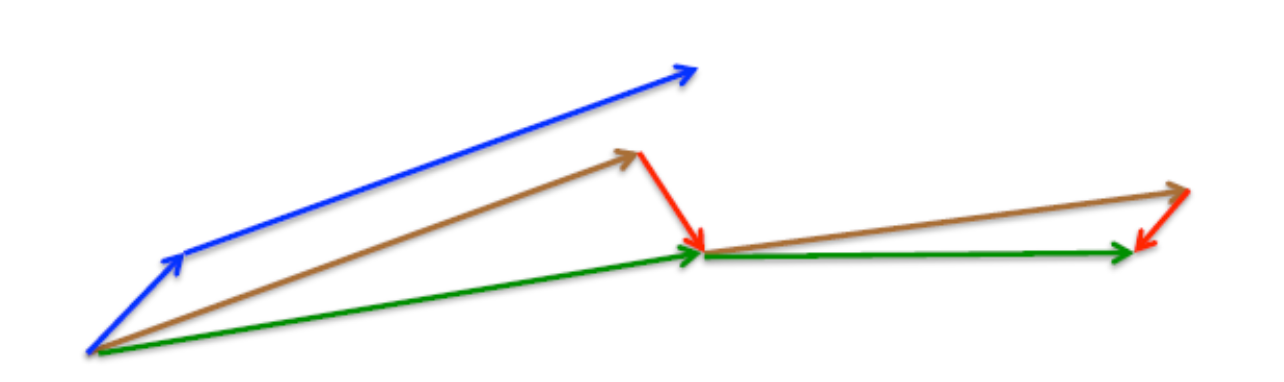
\includegraphics[width=0.55\linewidth]{figures/cf05_nesterov_vectors.png}
  \caption{Intuizione del Nesterov Accelerated Gradient. Il vettore marrone è il
           salto nella direzione accumulata, il rosso è la correzione, il verde è
           il gradiente accumulato risultante. I vettori blu rappresentano il
           percorso del momentum standard.}
  \label{fig:nesterov}
\end{figure}

\paragraph{Perché il momentum funziona?}
Esistono due spiegazioni complementari:

\begin{description}
  \item[Accelerazione] Con Nesterov è dimostrabile una convergenza accelerata su
        problemi \emph{convessi}. Per reti neurali la prova non si applica
        direttamente, e l'accelerazione regge solo su superfici quadratiche. In
        più, l'accelerazione non funziona bene in presenza di rumore stocastico.
  \item[Noise Smoothing] Ragione probabilmente più importante in pratica: il
        momentum è un \emph{running average} dei gradienti. Dove SGD richiederebbe
        di mediare molti aggiornamenti prima di fare un passo, il momentum lo fa
        automaticamente, rendendo ogni singolo aggiornamento una buona
        approssimazione della direzione corretta.
\end{description}

In sintesi, sia l'accelerazione che il noise smoothing contribuiscono alle buone
prestazioni del momentum SGD. Il noise smoothing evita il rimbalzamento sul
"pavimento" del minimo (bottom of the valley), mentre l'accelerazione velocizza
la discesa nelle regioni a bassa curvatura.

%------------------------------------------------------------
\section{Learning Rate Adattativi Separati}
\label{sec:adaptive-lr}

\subsection{Motivazione}
\label{subsec:adaptive-lr-motivation}

In una rete multi-layer i learning rate ottimali possono variare molto tra i
pesi:

\begin{itemize}
  \item Le ampiezze dei gradienti sono spesso molto diverse tra i layer,
        specialmente con pesi iniziali piccoli.
  \item Il fan-in di un'unità determina l'entità dell'effetto di overshoot
        causato dalla modifica simultanea di molti pesi in ingresso.
\end{itemize}

La strategia è usare un \textbf{learning rate globale} (impostato a mano)
moltiplicato per un \textbf{guadagno locale} $g_{ij}(t)$ determinato
empiricamente per ogni peso.

\subsection{Determinazione dei Guadagni Locali}
\label{subsec:local-gains}

Si parte da $g_{ij}(t_0) = 1$ per ogni peso. Poi, ad ogni step:

\begin{equation}
  \Delta w_{ij} = -\epsilon\, g_{ij}\, \frac{\partial E}{\partial w_{ij}}
\end{equation}

\begin{equation}
  g_{ij}(t) =
  \begin{cases}
    g_{ij}(t-1) + 0.05
      & \text{se } \dfrac{\partial E}{\partial w_{ij}}(t)\cdot
                   \dfrac{\partial E}{\partial w_{ij}}(t-1) > 0 \\[8pt]
    g_{ij}(t-1) \times 0.95
      & \text{altrimenti}
  \end{cases}
\end{equation}

Aumenti additivi e decrementi moltiplicativi garantiscono che i grandi guadagni
decadano rapidamente non appena iniziano le oscillazioni. I guadagni vengono
limitati in un intervallo ragionevole (es.\ $[0.1,\, 10]$ oppure $[0.01,\, 100]$).

\begin{tcolorbox}[colback=blue!5!white, colframe=blue!50!black, title=Analogia: AIMD nel controllo della congestione TCP]
Il meccanismo di aumento additivo e decremento moltiplicativo (AIMD) è lo stesso
principio usato nel controllo della congestione TCP: aumenta linearmente la
finestra di congestione finché non si verifica una perdita, poi la dimezza.
Questo garantisce robustezza e veloce recupero dalle oscillazioni.
\end{tcolorbox}

\paragraph{Combinare con il momentum.}
I learning rate adattativi possono essere combinati con il momentum usando
l'accordo di segno tra il gradiente corrente e la velocità del peso
(Jacobs, 1989). Nota che i learning rate adattativi gestiscono solo effetti
allineati agli assi (derivate parziali), mentre il momentum non dipende
dall'allineamento degli assi.

%------------------------------------------------------------
\section{rprop e rmsprop}
\label{sec:rprop-rmsprop}

\subsection{rprop: Solo il Segno del Gradiente}
\label{subsec:rprop}

Quando l'ampiezza del gradiente varia molto tra pesi diversi e durante
l'addestramento, è difficile scegliere un unico learning rate globale. Per il
\textbf{full batch learning} si può ovviare usando solo il \emph{segno} del
gradiente:

\begin{itemize}
  \item Tutti gli aggiornamenti di peso hanno la stessa ampiezza.
  \item Si esce rapidamente dalle regioni a gradiente quasi nullo (plateau).
\end{itemize}

\textbf{rprop} combina l'uso del solo segno del gradiente con l'adattamento
della dimensione del passo per ogni peso separatamente:

\begin{itemize}
  \item Se i segni degli ultimi due gradienti \emph{concordano}: moltiplica la
        dimensione del passo per $1.2$.
  \item Altrimenti: moltiplica per $0.5$.
  \item Limita la dimensione del passo nell'intervallo $[10^{-6},\, 50]$.
\end{itemize}

\paragraph{Perché rprop non funziona con i mini-batch.}
SGD media implicitamente i gradienti su mini-batch successivi (quando il
learning rate è piccolo). rprop, invece, aggiorna la dimensione del passo sulla
base del \emph{segno} in ogni mini-batch separatamente. Se un peso riceve
gradiente $+0.1$ per nove mini-batch e $-0.9$ per uno, rprop incrementerebbe il
peso nove volte e lo decrementerà una sola volta, portando a un'esplosione del
peso. Questo motiva la necessità di rmsprop.

\subsection{rmsprop: Versione Mini-Batch di rprop}
\label{subsec:rmsprop}

\textbf{rmsprop} mantiene una media mobile del quadrato del gradiente per ogni
peso e divide il gradiente per la radice di questa media:

\begin{equation}
  \text{MeanSquare}(w, t) =
    0.9\;\text{MeanSquare}(w, t-1) + 0.1\left(\frac{\partial E}{\partial w}\right)^2,
\end{equation}

\begin{equation}
  \Delta w = -\frac{\eta}{\sqrt{\text{MeanSquare}(w,t)}}\;\frac{\partial E}{\partial w}.
\end{equation}

Dividere per $\sqrt{\text{MeanSquare}(w,t)}$ normalizza il gradiente rispetto
alla sua ampiezza recente, ottenendo l'effetto di rprop ma in modo compatibile
con i mini-batch. I valori suggeriti da Hinton sono $\gamma = 0.9$ e
$\eta = 0.001$.

%------------------------------------------------------------
\section{Metodi Adattativi Avanzati}
\label{sec:advanced-adaptive}

\subsection{Adagrad}
\label{subsec:adagrad}

\textbf{Adagrad} adatta il learning rate a ciascun parametro, effettuando
aggiornamenti più grandi per parametri rari e più piccoli per quelli frequenti.
Definendo $g_{t,i} = \nabla_\theta J(\theta_{t,i})$, l'aggiornamento SGD
standard diventa:

\begin{equation}
  \theta_{t+1,i} = \theta_{t,i} - \frac{\eta}{\sqrt{G_{t,ii} + \epsilon}}
                   \cdot g_{t,i},
\end{equation}

dove $G_t \in \mathbb{R}^{d \times d}$ è una matrice diagonale il cui elemento
$(i,i)$ è la \textbf{somma dei quadrati di tutti i gradienti passati} rispetto
a $\theta_i$ fino al passo $t$, e $\epsilon \approx 10^{-8}$ evita la
divisione per zero.

\paragraph{Vantaggi e limiti.}
Adagrad elimina la necessità di regolare manualmente il learning rate (default
$0.01$). Il limite principale è che la somma dei gradienti al quadrato cresce
monotonamente: il learning rate si riduce fino a diventare infinitesimo,
bloccando l'apprendimento.

\subsection{Adadelta}
\label{subsec:adadelta}

\textbf{Adadelta} risolve il problema di Adagrad sostituendo la somma
cumulativa dei quadrati del gradiente con una \emph{media esponenzialmente
decrescente}:

\begin{equation}
  E[g^2]_t = \gamma\, E[g^2]_{t-1} + (1-\gamma)\, g_t^2.
\end{equation}

L'aggiornamento diventa:

\begin{equation}
  \theta_{t+1,i} = \theta_{t,i} - \frac{\text{RMS}[\Delta\theta]_{t-1}}
                                        {\text{RMS}[g]_t}\, g_t,
\end{equation}

dove $\text{RMS}[g]_t = \sqrt{E[g^2]_t + \epsilon}$ e
$\text{RMS}[\Delta\theta]_{t-1}$ è la radice del mean square degli aggiornamenti
passati (anch'esso calcolato con media esponenziale). In questo modo il learning
rate viene eliminato dall'equazione e non deve essere impostato.

\paragraph{Relazione con rmsprop.}
RMSprop e Adadelta sono stati sviluppati indipendentemente nello stesso periodo
per risolvere lo stesso problema. RMSprop corrisponde esattamente al primo
vettore di aggiornamento di Adadelta.

\subsection{Adam: Adaptive Moment Estimation}
\label{subsec:adam}

\textbf{Adam} \citep{kingma2014adam} combina l'idea di rmsprop (media del quadrato
dei gradienti) con quella del momentum (media dei gradienti), mantenendo stime
del \emph{primo momento} (media) e del \emph{secondo momento non centrato}
(varianza) dei gradienti:

\begin{align}
  m_t &= \beta_1\, m_{t-1} + (1-\beta_1)\, g_t, \\
  v_t &= \beta_2\, v_{t-1} + (1-\beta_2)\, g_t^2.
\end{align}

Poiché $m_0 = v_0 = \mathbf{0}$, le stime sono distorte verso zero nelle prime
iterazioni. Si correggono con:

\begin{equation}
  \hat{m}_t = \frac{m_t}{1 - \beta_1^t}, \qquad
  \hat{v}_t = \frac{v_t}{1 - \beta_2^t}.
\end{equation}

L'aggiornamento finale è:

\begin{equation}
  \theta_{t+1} = \theta_t - \frac{\eta}{\sqrt{\hat{v}_t} + \epsilon}\,\hat{m}_t.
\end{equation}

I valori di default suggeriti dagli autori sono $\beta_1 = 0.9$,
$\beta_2 = 0.999$, $\epsilon = 10^{-8}$.

\paragraph{Interpretazione.}
Quando i gradienti rimangono approssimativamente costanti (discesa uniforme),
la varianza è quasi nulla e $v_t \approx m_t^2$, quindi
$\hat{m}_t / \sqrt{\hat{v}_t} \approx 1$: il passo è dell'ordine di $\eta$.
Quando i gradienti cambiano rapidamente, $\sqrt{\hat{v}_t} \gg \hat{m}_t$ e il
passo diventa molto più piccolo di $\eta$. Adam adatta quindi la dimensione del
passo in modo automatico per ciascun peso.

\begin{figure}[H]
  \centering
  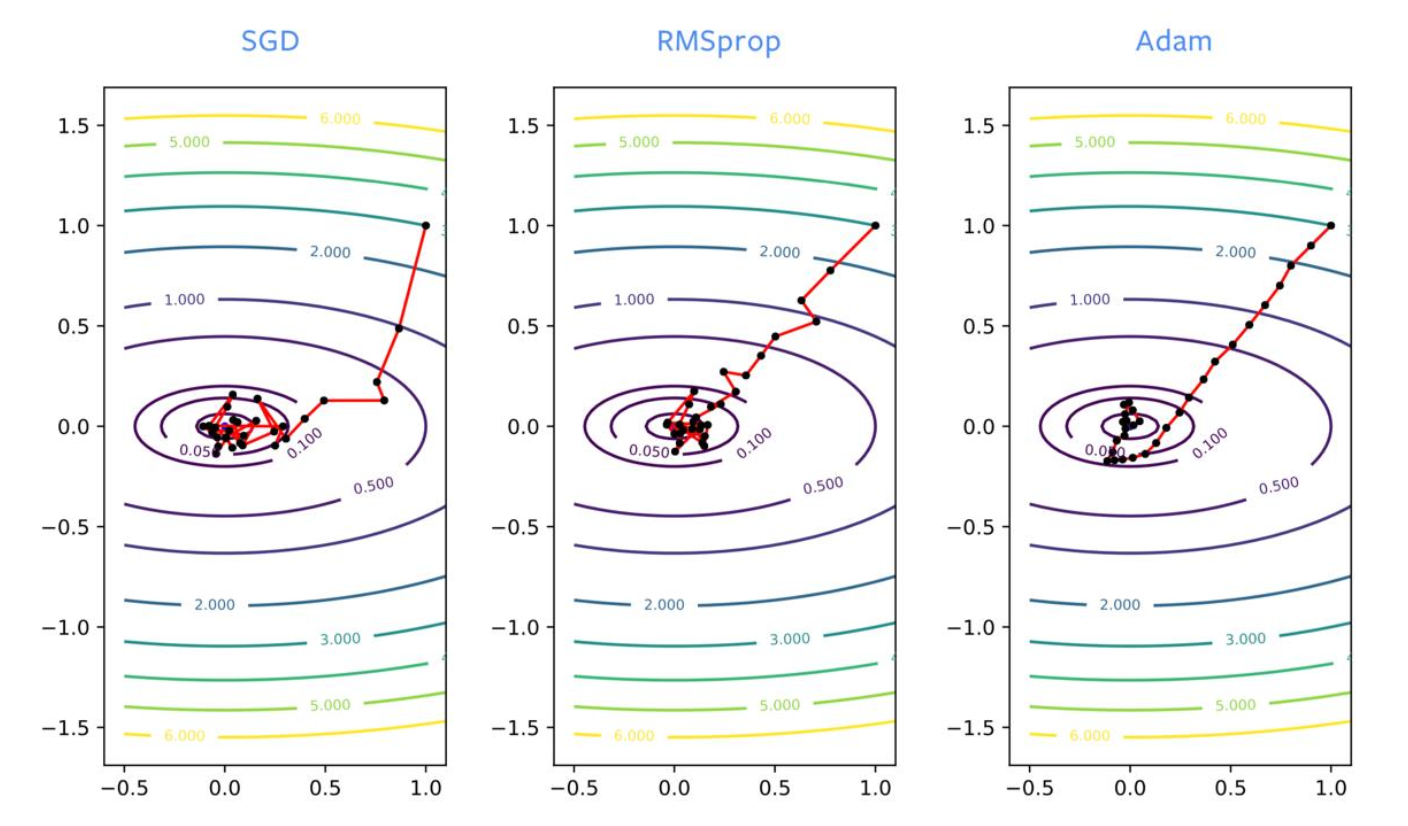
\includegraphics[width=0.88\linewidth]{figures/cf05_sgd_rmsprop_adam.png}
  \caption{Confronto delle traiettorie di SGD, RMSprop e Adam sulla stessa
           superficie di errore. Adam converge in modo più diretto verso il
           minimo grazie alla combinazione di momentum e normalizzazione
           adattiva.}
  \label{fig:sgd_vs_adam}
\end{figure}

\subsubsection{Limitazioni di Adam}
\label{subsubsec:adam-limits}

\begin{itemize}
  \item Su problemi semplici è dimostrabile che Adam \textbf{non converge}.
  \item Tende a produrre \textbf{errori di generalizzazione} maggiori rispetto a
        SGD, specialmente in computer vision: trovare il minimo locale più vicino
        (invece del minimo "piatto" favorito da SGD) porta a minori capacità di
        generalizzazione.
  \item Richiede \textbf{3 buffer} invece di 1 (pesi, $m_t$, $v_t$): per modelli
        da miliardi di parametri questo può diventare limitante in memoria.
  \item Sono necessari 2 iperparametri di momentum da regolare invece di 1.
\end{itemize}

\subsection{AdamW: Adam con Weight Decay Corretto}
\label{subsec:adamw}

Le librerie di deep learning implementano tipicamente la \emph{L2
regularization} aggiungendo $\lambda\, w$ al gradiente prima dell'aggiornamento.
Tuttavia questo non è equivalente al weight decay per gli ottimizzatori
adattativi: il termine di regolarizzazione viene normalizzato da $\sqrt{v_t}$,
quindi i pesi con gradienti grandi vengono regolarizzati \emph{meno} di quelli
con gradienti piccoli. \textbf{AdamW} separa il weight decay dall'aggiornamento
adattivo:

\begin{equation}
  \mathbf{x}_t \leftarrow \mathbf{x}_{t-1}
    - \eta_t \left(\frac{\alpha\,\hat{m}_t}{\sqrt{\hat{v}_t} + \epsilon}\right)
    - \eta_t\, w\, \mathbf{x}_{t-1}.
\end{equation}

Il termine di regolarizzazione $w\,\mathbf{x}_{t-1}$ è proporzionale al solo
valore del peso e non viene influenzato dalla normalizzazione adattiva,
replicando il comportamento del weight decay in SGD e migliorando la
generalizzazione.

\subsection{Lion: EvoLved Sign Momentum}
\label{subsec:lion}

\textbf{Lion} \citep{chen2023lion} è un ottimizzatore scoperto tramite
\emph{program search} (ricerca evolutiva sullo spazio dei programmi). Richiede
meno memoria di Adam (mantiene solo il momentum, non il secondo momento) e
produce aggiornamenti di ampiezza uniforme grazie all'operazione \texttt{sign}:

\begin{lstlisting}[language=Python, caption={Pseudocodice di Lion.}, label={lst:lion}]
def train(weight, gradient, momentum, lr):
    update   = interp(gradient, momentum, beta1)  # (1-b1)*m + b1*g
    update   = sign(update)
    momentum = interp(gradient, momentum, beta2)
    update   = update + weight * lambda_wd         # weight decay
    update   = update * lr
    return update, momentum
\end{lstlisting}

Le prestazioni di Lion crescono con la dimensione del mini-batch e richiedono un
learning rate più piccolo rispetto ad Adam a causa della norma maggiore prodotta
dalla funzione \texttt{sign}.

%------------------------------------------------------------
\section{Metodi di Secondo Ordine}
\label{sec:second-order}

\subsection{Riduzione dell'Errore e Rapporto Gradiente/Curvatura}
\label{subsec:gradient-curvature}

La riduzione massima dell'errore percorrendo una direzione $\mathbf{d}$ dipende
dal \textbf{rapporto gradiente/curvatura}. Una buona direzione ha un rapporto
elevato anche se il gradiente è piccolo. Per trovare queste direzioni si può
usare la matrice di curvatura (Hessiana):

\begin{equation}
  H_{i,j} = \frac{\partial^2 f}{\partial x_i \partial x_j}.
\end{equation}

\begin{description}
  \item[Gradiente] Vettore delle derivate prime di un campo scalare.
  \item[Jacobiano] Matrice dei gradienti per le componenti di un campo vettoriale
        ($J_{i,j} = \partial F_i / \partial x_j$).
  \item[Hessiana] Matrice delle derivate miste di secondo ordine di un campo
        scalare.
\end{description}

\subsection{Metodo di Newton}
\label{subsec:newton}

Il metodo di Newton moltiplica il vettore del gradiente per l'inversa della
matrice di curvatura $H$:

\begin{equation}
  \Delta \mathbf{w} = -\epsilon\, H(\mathbf{w})^{-1}\, \frac{dE}{d\mathbf{w}}.
\end{equation}

Su una superficie quadratica reale converge al minimo in un unico passo. Il
problema pratico è che con un milione di pesi la matrice di curvatura ha un
trilione di termini: \textbf{inverirla è computazionalmente intrattabile}.

\paragraph{Matrici di curvatura.}
Ogni elemento della matrice specifica come il gradiente in una direzione cambia
spostandosi in un'altra. I termini fuori diagonale corrispondono alle
\emph{torsioni} della superficie di errore. La ragione per cui la discesa del
gradiente produce zig-zag è che aggiornare un peso muta il gradiente di tutti
gli altri.

\subsection{Hessian-Free Optimization e Gradiente Coniugato}
\label{subsec:hessian-free}

Il metodo \textbf{Hessian-Free} (HF) approssima la matrice di curvatura e,
assumendo che quell'approssimazione sia corretta, minimizza l'errore usando il
\textbf{gradiente coniugato} (CG). Poi aggiorna l'approssimazione e minimizza di
nuovo.

\paragraph{Gradiente Coniugato.}
Invece di invertire $H$ in un solo passo, CG usa una sequenza di passi ognuno
dei quali minimizza l'errore lungo una direzione:

\begin{itemize}
  \item Ogni nuova direzione è \emph{coniugata} alle precedenti: muoversi in
        essa non altera i gradienti nelle direzioni già ottimizzate.
  \item Dopo $N$ passi è garantita la convergenza al minimo di una superficie
        quadratica $N$-dimensionale.
  \item Applicato a superfici non quadratiche (CG non lineare) funziona comunque
        bene nella pratica.
\end{itemize}

L'ottimizzatore HF usa CG sulla superficie quadratica approssimata (dove CG è
ottimale). Per le RNN è importante aggiungere un vincolo che impedisce di
modificare troppo le attività nascoste da un'iterazione all'altra.

%------------------------------------------------------------
\section{Riepilogo dei Metodi di Ottimizzazione}
\label{sec:optim-summary}

\begin{table}[H]
  \centering
  \caption{Guida alla scelta dell'ottimizzatore.}
  \label{tab:optim_guide}
  \small
  \begin{tabular}{lll}
    \toprule
    \textbf{Scenario} & \textbf{Ottimizzatore} & \textbf{Note} \\
    \midrule
    Dataset piccolo ($\leq$10k) / bassa ridondanza
      & Full-batch (CG, L-BFGS, rprop)
      & Convergenza precisa \\
    Dataset grande e ridondante
      & Mini-batch SGD + Momentum
      & Default per CV \\
    Gradient sparso / NLP / embedding
      & Adam / AdamW
      & Adattività per feature rare \\
    Modelli grandi, generalizzazione critica
      & AdamW o SGD + momentum
      & AdamW corregge weight decay \\
    Memoria limitata, batch grande
      & Lion
      & Un solo buffer di stato \\
    \bottomrule
  \end{tabular}
\end{table}

\paragraph{Regole operative.}
\begin{enumerate}
  \item Inizializzare i pesi con \textbf{Xavier/Glorot} (sigmoide/tanh) o
        \textbf{He} (ReLU); mai inizializzare a zero tutti i pesi hidden.
  \item Normalizzare gli input (media zero, varianza unitaria) o usare Batch
        Normalization per accelerare la convergenza.
  \item Per reti grandi preferire \textbf{AdamW} come default; passare a SGD
        con momentum e cosine annealing per massimizzare la generalizzazione.
  \item Non abbassare il learning rate troppo presto: attendere che la loss si
        sia stabilizzata su un plateau.
  \item Usare mini-batch bilanciati tra le classi (cfr.\ Sezione
        \ref{subsec:redundancy}) e limitare la dimensione del mini-batch
        tenendo conto che batch più grandi richiedono learning rate più alti
        (linear scaling rule).
  \item Per i learning rate adattativi limitare sempre i guadagni locali in un
        intervallo ragionevole e usare mini-batch grandi per ridurre il rumore
        nelle stime dei segni del gradiente.
\end{enumerate}

Come sottolinea \citet{bishop2024}, non esiste una ricetta universale perché le
reti neurali differiscono enormemente (reti molto profonde, reti ricorrenti,
reti wide-shallow) e i task pongono requisiti diversi (accuratezza dei pesi,
presenza di feature rare, …). La scelta dell'ottimizzatore va quindi fatta
considerando congiuntamente architettura, dataset e obiettivo di generalizzazione.
